\documentclass[a4paper,12pt]{article}
%%%%%%%%%%%%%%%%%%%%%%%%%%%%%%%%%%%%%%%%%%%%%%%%%%%%%%%%%%%%%%%%%%%%%%%%%%%%%%%%%%%%%%%%%%%%%%%%%%%%%%%%%%%%%%%%%%%%%%%%%%%%%%%%%%%%%%%%%%%%%%%%%%%%%%%%%%%%%%%%%%%%%%%%%%%%%%%%%%%%%%%%%%%%%%%%%%%%%%%%%%%%%%%%%%%%%%%%%%%%%%%%%%%%%%%%%%%%%%%%%%%%%%%%%%%%
\usepackage{eurosym}
\usepackage{vmargin}
\usepackage{amsmath}
\usepackage{graphics}
\usepackage{epsfig}
\usepackage{subfigure}
\usepackage{fancyhdr}
\usepackage{listings}
\usepackage{framed}
\usepackage{graphicx}
\usepackage{amsmath}
\usepackage{chngpage}
%\usepackage{bigints}

%\setcounter{MaxMatrixCols}{10}

\begin{document}
	\large
%	%%-
%nbviewer
%FAQ
%IPython
%Jupyter
%bokeh-notebooks   tutorial
 	
\section*{Bokeh Tutorial — Adding Interactions}

\subsection*{Preliminaries}
\begin{framed}
\begin{verbatim}

from bokeh.io import gridplot, output_notebook, show
from bokeh.plotting import figure
output_notebook()
# BokehJS successfully loaded.
	
\end{verbatim}
\end{framed}
%===========================================================================================================%	

\newpage
\subsection*{Simple Layouts}
\begin{itemize}
\item In order to add widgets or have multiple plots that are linked together, you must first be able to create documents that contain these separate objects. \item \textbf{OLD:} In the upcoming 0.9.1 release (Jul 2015), it will be possible to easily accomplish this in your own custom templates using \texttt{bokeh.embed.components}. 
\item \textbf{OLD:} For now you, Bokeh provides simple layout capability for grid plots, VBoxes, and HBoxes (than can be nested).
\end{itemize}


An example using \texttt{gridplot} is shown below:
\begin{framed}
	\begin{verbatim}

x = list(range(11))
y0, y1, y2 = x, [10-i for i in x], [abs(i-5) for i in x]

# create a new plot
s1 = figure(width=250, plot_height=250)
s1.circle(x, y0, size=10, color="navy", alpha=0.5)

# create another one
s2 = figure(width=250, height=250)
s2.triangle(x, y1, size=10, color="firebrick", alpha=0.5)

# create and another
s3 = figure(width=250, height=250)
s3.square(x, y2, size=10, color="olive", alpha=0.5)

# put all the plots in an HBox
p = gridplot([[s1, s2, s3]], toolbar_location=None)

# show the results
show(p)

# EXERCISE: create a gridplot of your own
	
\end{verbatim}
\end{framed}
\newpage
\begin{figure}[h!]
\centering
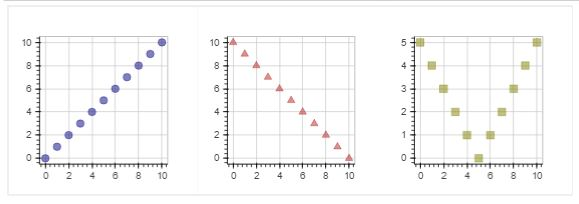
\includegraphics[width=1.1\linewidth]{images/06-interactions-tut-01}

\end{figure}



Bokeh also provides the vplot and hplot functions to arrange plot objects in vertical or horizontal layouts.

\bigskip
\noindent EXERCISE: use \texttt{vplot} to arrange a few plots vertically
\subsection*{Linked Interactions}
It is possible to link various interactions between different Bokeh plots. For instance, the ranges of two (or more) plots can be linked, so that when one of the plots is panned (or zoomed, or otherwise has its range changed) the other plots will update in unison. It is also possible to link selections between two plots, so that when items are selected on one plot, the corresponding items on the second plot also become selected.
\begin{figure}[h!]
\centering
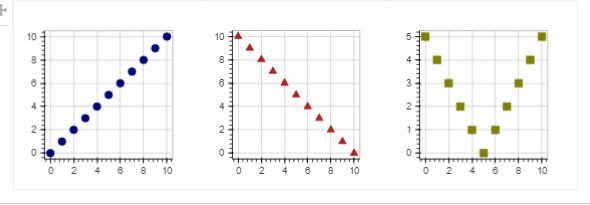
\includegraphics[width=0.7\linewidth]{images/06-interactions-tut-02}
\end{figure}

\begin{itemize}
	\item Linked Panning 
	\item Linked Brushing
\end{itemize}
%=========================================================================================================== %
\newpage
\subsection*{Linked panning}
Linked panning (when mulitple plots have ranges that stay in sync) is simple to spell with Bokeh. You simply share the approrpate range objects between two (or more) plots. The example below shows how to accomplish this by linking the ranges of three plots in various ways:
\begin{framed}
	\begin{verbatim}

# create a new plot
s1 = figure(width=250, plot_height=250, title=None)
s1.circle(x, y0, size=10, color="navy", alpha=0.5)

# create a new plot and share both ranges
s2 = figure(width=250, height=250, x_range=s1.x_range, y_range=s1.y_range, title=None)
s2.triangle(x, y1, size=10, color="firebrick", alpha=0.5)

# create a new plot and share only one range
s3 = figure(width=250, height=250, x_range=s1.x_range, title=None)
s3.square(x, y2, size=10, color="olive", alpha=0.5)

p = gridplot([[s1, s2, s3]], toolbar_location=None)

# show the results
show(p)
\end{verbatim}
\end{framed}

\begin{figure}
\centering
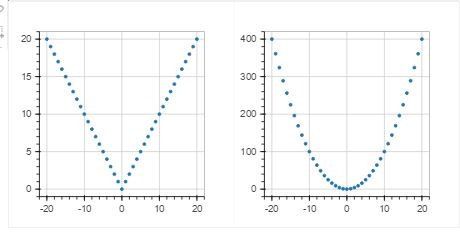
\includegraphics[width=0.7\linewidth]{images/06-interactions-tut-03}
\end{figure}

EXERCISE: create two plots in a gridplot, and link their ranges
	


%==================================================================== %
\subsection{Linked brushing}
\begin{itemize}
\item Linking selections is accomplished in a similar way, by sharing data sources between plots. 
\item Note that normally with \texttt{bokeh.plotting} and \texttt{bokeh.charts} creating a default data source for simple plots is handled automatically. 
\item However to share a data source, we must create them by hand and pass them explicitly. This is illustrated in the example below:
\end{itemize}

\begin{framed}
	\begin{verbatim}
	
In [8]:
from bokeh.models import ColumnDataSource

x = list(range(-20, 21))
y0, y1 = [abs(xx) for xx in x], [xx**2 for xx in x]

# create a column data source for the plots to share
source = ColumnDataSource(data=dict(x=x, y0=y0, y1=y1))

TOOLS = "box_select,lasso_select,help"

# create a new plot and add a renderer
left = figure(tools=TOOLS, width=300, height=300)
left.circle('x', 'y0', source=source)

# create another new plot and add a renderer
right = figure(tools=TOOLS, width=300, height=300)
right.circle('x', 'y1', source=source)

p = gridplot([[left, right]])

show(p)
 
\end{verbatim}
\end{framed}
\begin{figure}[h!]
	\centering
	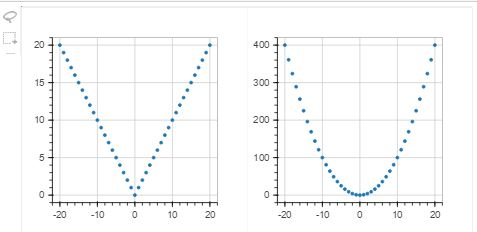
\includegraphics[width=0.7\linewidth]{images/06-interactions-tut-04}
\end{figure}

EXERCISE: create two plots in a gridplot, and link their data sources

%========================================================== %
\newpage
\subsection{Hover Tools}
\begin{itemize}
\item Bokeh has a Hover Tool that allows additional information to be displayed in a popup whenever the uer howevers over a specific glyph. 
\item Basic hover tool configuration amounts to providing a list of (name, format) tuples. 
%\item The full details can be found in the User's Guide here.
\end{itemize}


The example below shows some basic usage of the Hover tool with a circle glyph:

\begin{framed}
\begin{verbatim}

from bokeh.models import HoverTool

source = ColumnDataSource(
        data=dict(
            x=[1, 2, 3, 4, 5],
            y=[2, 5, 8, 2, 7],
            desc=['A', 'b', 'C', 'd', 'E'],
        )
    )

hover = HoverTool(
        tooltips=[
            ("index", "$index"),
            ("(x,y)", "($x, $y)"),
            ("desc", "@desc"),
        ]
    )

p = figure(plot_width=400, plot_height=400, tools=[hover], title="Mouse over the dots")

p.circle('x', 'y', size=20, source=source)

show(p)

\end{verbatim}
\end{framed}

\begin{figure}
\centering
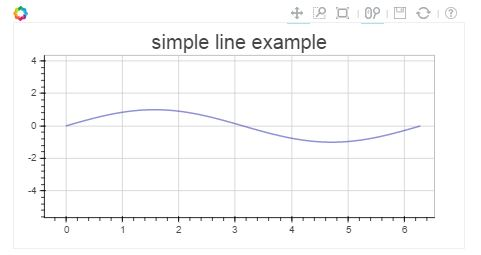
\includegraphics[width=0.7\linewidth]{images/06-interactions-tut-05}
\caption{}
\label{fig:06-interactions-tut-05}
\end{figure}
%=========================================================================================================== %
\subsection{Ipython Interactors}
\begin{itemize}
\item It is possible to use native IPython notebook interactors together with Bokeh. 
\item In the interactor update function, the \texttt{push\_notebook} method can be used to update a data source (presumably based on the iteractor widget values) to cause a plot to update.

\item \textbf{Warning:} The current implementation of \texttt{push\_notebook} leaks memory. It is suitable for interactive exploration but not for long-running or streaming use cases. The problem will be resolved in future releases.
\end{itemize}

The example below shows a "\texttt{trig function}" exporer using IPython interactors:

\begin{framed}
\begin{verbatim}
import numpy as np
from bokeh.models import Line

x = np.linspace(0, 2*np.pi, 2000)
y = np.sin(x)

source = ColumnDataSource(data=dict(x=x, y=y))

p = figure(title="simple line example", 
     plot_height=300, plot_width=600, y_range=(-5, 5))
     
p.line(x, y, color="#2222aa", alpha=0.5, 
     line_width=2, source=source, name="foo")

def update(f, w=1, A=1, phi=0):
    if   f == "sin": func = np.sin
    elif f == "cos": func = np.cos
    elif f == "tan": func = np.tan
    source.data['y'] = A * func(w * x + phi)
    source.push_notebook()

show(p)
\end{verbatim}
\end{framed}

\begin{figure}
\centering
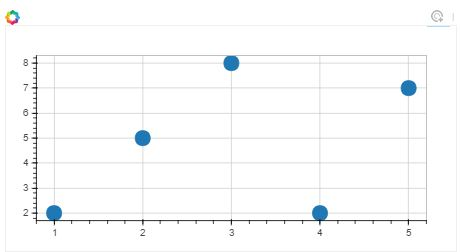
\includegraphics[width=0.7\linewidth]{images/06-interactions-tut-06}
\end{figure}

%======================================================= %	
\begin{framed}
	\begin{verbatim}
	
In [11]:
from ipywidgets import interact
interact(update, f=["sin", "cos", "tan"], w=(0,10, 0.1), A=(0,5, 0.1), phi=(0, 10, 0.1))
None
Out[11]:
<function __main__.update>
Bokeh Widgets and Callbacks
	
\end{verbatim}
\end{framed}

%======================================================== %
\newpage
\subsection*{Adding Widgets}
\begin{itemize}
\item Bokeh supports direct integration with a small basic widget set. 
\item These can be used in conjunction with a Bokeh Server, or with CustomJS models to add more interactive capability to your documents. 
\item You can see a complete list, with example code in the Adding Widgets section of the User's Guide.
\end{itemize}


To use the widgets, include them in a layout like you would a plot object:
\begin{framed}
	\begin{verbatim}

from bokeh.models.widgets import Slider
from bokeh.io import vform

slider = Slider(start=0, end=10, value=1, step=.1, title="foo")

show(vform(slider))

\end{verbatim}
\end{framed}
\noindent \textbf{EXERCISE:} create and show a Select widget 
%=========================================================================================================== %
\subsection{Callbacks for widgets}
\begin{itemize}
\item Widgets that have values associated can have small JavaScript actions attached to them. 
\item These actions (also referred to as "callbacks") are executed whenever the widget's value is changed. 
\item In order to make it easier to refer to specific Bokeh models (e.g., a data source, or a glyhph) from JavaScript, the CustomJS obejct also accepts a dictionary of "args" that map names to Python Bokeh models. 
\item The corresponding JavaScript models are made available automaticaly to the CustomJS code.
\end{itemize}


And example below shows an action attached to a slider that updates a data source whenever the slider is moved:
\begin{framed}
	\begin{verbatim}
from bokeh.io import vform
from bokeh.models import CustomJS, ColumnDataSource, Slider

x = [x*0.005 for x in range(0, 200)]
y = x

source = ColumnDataSource(data=dict(x=x, y=y))

plot = figure(plot_width=400, plot_height=400)
plot.line('x', 'y', source=source, line_width=3, line_alpha=0.6)

callback = CustomJS(args=dict(source=source), code="""
    var data = source.get('data');
    var f = cb_obj.get('value')
    x = data['x']
    y = data['y']
    for (i = 0; i < x.length; i++) {
        y[i] = Math.pow(x[i], f)
    }
    source.trigger('change');
""")

slider = Slider(start=0.1, end=4, value=1, step=.1, title="power", callback=callback)

layout = vform(slider, plot)

show(layout)
power:  
1
	
\end{verbatim}
\end{framed}
 	

%=========================================================================================================== %
\newpage
\subsection*{Calbacks for selections}
\begin{itemize}
\item It's also possible to make JavaScript actions that execute whenever a user selection (e.g., box, point, lasso) changes. 
\item This is done by attaching the same kind of CustomJS object to whatever data source the selection is made on.
\end{itemize}

The example below is a bit more sophisticaed, and demonstrates updating one glyphs data source in response to another glyph's selection:
\begin{framed}
\begin{verbatim}
In [13]:
from random import random

x = [random() for x in range(500)]
y = [random() for y in range(500)]
color = ["navy"] * len(x)

s = ColumnDataSource(data=dict(x=x, y=y, color=color))
p = figure(plot_width=400, plot_height=400, tools="lasso_select", title="Select Here")
p.circle('x', 'y', color='color', size=8, source=s, alpha=0.4)

s2 = ColumnDataSource(data=dict(ym=[0.5, 0.5]))
p.line(x=[0,1], y='ym', color="orange", line_width=5, alpha=0.6, source=s2)

s.callback = CustomJS(args=dict(s2=s2), code="""
    var inds = cb_obj.get('selected')['1d'].indices;
    var d = cb_obj.get('data');
    var ym = 0
    
    if (inds.length == 0) { return; }
    
    for (i = 0; i < d['color'].length; i++) {
        d['color'][i] = "navy"
    }
    for (i = 0; i < inds.length; i++) {
        d['color'][inds[i]] = "firebrick"
        ym += d['y'][inds[i]]
    }
    
    ym /= inds.length
    s2.get('data')['ym'] = [ym, ym]
    
    cb_obj.trigger('change');
    s2.trigger('change');
""")

show(p)
	
\end{verbatim}
\end{framed}
 
 %=========================================================================================================== %
\begin{figure}
\centering
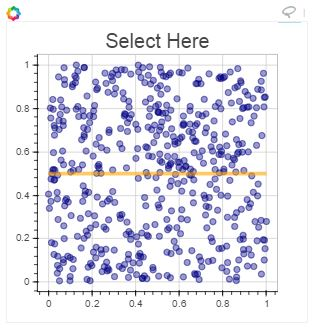
\includegraphics[width=0.7\linewidth]{images/06-interactions-tut-callbacksforselections}
\end{figure}

 \end{document}